% GENERATED FROM typst/manual/sections/09_prediction_test_fixture_registry.typ BY scripts/typ2tex.py (v1.0.0) — DO NOT EDIT.
% Edit canonical Typst under typst/ and regenerate with: python3 scripts/typ2tex.py --root . --outdir latex

\section{Prediction-Test Fixture Registry}\label{manual:prediction-test-registry}

\paragraph{Reading the registry.}
Data support describes the supplied coordinates. Record completeness lists
the supplied calculation/comparison stages; replay requires their bound
producer and operands; physical evidence requires source uncertainty and a
properly classified comparison. These are separate properties. Each row
below links through its application card to the common method in
\secref{manual:calculation-spine}; a carried map or aggregate is not promoted
by a source-only replay.

\aodnoteblock{Scope}{This registry records completion fields for manual fixtures and comparisons. Rows carry their data-support class, active fields, required A$\Omega$ calculation, and audit artifact.}

{\footnotesize
\begin{longtable}{>{\raggedright\arraybackslash}p{0.160\linewidth}>{\raggedright\arraybackslash}p{0.080\linewidth}>{\raggedright\arraybackslash}p{0.160\linewidth}>{\raggedright\arraybackslash}p{0.250\linewidth}>{\raggedright\arraybackslash}p{0.180\linewidth}}
\caption{Prediction-test fixture registry.}\label{tab:manual-prediction-test-registry} \\
\toprule
Record & Class & Active fields & Required A$\Omega$ calculation & Artifact \\
\midrule
\endfirsthead
\toprule
Record & Class & Active fields & Required A$\Omega$ calculation & Artifact \\
\midrule
\endhead
Hydrogen shell radii & O0 & target rows & shell-ratio record for $S_n$ & radius-ratio table \\
Hydrogen shell energies & O0 & target rows & $\Delta\hat{P}^D$, ratio, target & Lyman / Balmer / Paschen tables \\
Short-window $1:2:7$ & D0 & integer fixture fields & $P^D,\Delta^{\mathrm{close}},X_{\mathrm{shedding}}$ & closure table \\
Short-window $1:2:9$ & D0 & integer fixture fields & $P^D,C^{\mathrm{close}},X_{\mathrm{shedding}}$ & surplus table \\
Toy 1 field-ring fixture & D0 & integer comparator bins & $T^0,C^{\times},T^{\times},O,\Delta^{\mathbb{Z}},\delta_3$ & $\delta_3$ fixture table \\
Neuronal-ring benchmark acquisition & L2 & acquisition fields & $\mathcal{S}_{\mathrm{neuro}},O_k$ & acquisition declaration \\
Electron & O0 & measured target rows & $\nu_{\AO},E_{\mathrm{ext}}$ for $1:2:6$ & external target declared \\
Muon & O0 & measured target rows & $\nu_{\AO},E_{\mathrm{ext}}$ for $1:2:8$ & external target declared \\
Tau & O0/D0 & measured target rows & $\nu_{\AO},E_{\mathrm{ext}}$ for $1:2:9_{\mathrm{yro}}$ / Dimonnanyro & surplus fixture + external target declared \\
Proton & O0 & measured target rows & $\nu_{\AO},E_{\mathrm{ext}}$ for $3:3:6$ & closed fixture + external target declared \\
Neutron & O0 & measured target rows & $\nu_{\AO},E_{\mathrm{ext}}$ for $3:4:6$ & closed fixture + external target declared \\
B / $B_s$ / $B_c$ & O0 & measured target rows & $\nu_{\AO},E_{\mathrm{ext}}$ for Ditrion records & debris fixture + external target declared \\
Boundary current & D0 & declared boundary/current fields & $\Phi,J,P^D,\mathbf{A}_F$ & substitution table \\
Field tunnelling hinge-slide fixture & D0 & integer fixture fields & $\operatorname{adm}(e_0;B|t)=0$, slide kernel, $\rho^D_{\omega}$, $T^D_{\mathrm{tunnel}}$ & D.E.C. ledger table \\
3D Brownian phase-cycle fixture & G3/D0 & 3D coordinate track fields & $z_i\in\mathbb{Z}^3$, $\Delta z_i^{(n)}$, $Q_i^{(n)}$, phase counts, octant counts, $\delta_3$ & 3D coordinate phase-cycle CSVs (Brownian application aliases), integer-ratio audit, and App.~\ref{manual:app:coordinate-phase-cycle-delta3} \\
Run-tumble tracer-current fixture & G3/D0 & mode $m_t$, selected channel $j_t$, sign $\sigma_t$, accumulated trace $h_t\in\mathbb{Z}^4$, projection $\pi_3(h_t)\in\mathbb{Z}^3$, $Q^2_{3D}$, $Q^2_4$, phase counts, octant counts, $\delta_3$ & $h_t=h_{t-1}+\sigma_t\mathbf{e}_{j_t}$, $z_t=\pi_3(h_t)$, $Q^2_{3D}$ and $Q^2_4$ audit calculations, phase-cycle and octant $\delta_3$ tallies & run-tumble trace CSV, phase-cycle $\delta_3$, octant $\delta_3$, integer-ratio audit, generated trace table, and App.~\ref{manual:app:coordinate-phase-cycle-delta3} \\
Mercury perihelion & O0 & observable-map target rows & observable-map value, target, error & solar table \\
Solar light bending & O0 & observable-map target rows & observable-map value, target, error & solar table \\
Solar redshift & O0 & observable-map target rows & observable-map value, target, error & solar table \\
Earth--Moon orbital shell & O0 & target data manifest & Moon distance, speed, period records require numeric A$\Omega$ values & NASA target record \\
Saturn ring-shell & O0 & target data manifest & ring-boundary and Cassini-division records require numeric A$\Omega$ values & NASA / ring-boundary target record \\
SPARC five-galaxy square-speed diagnostic & G0 & SPARC radial rows & $U_{\AO}(r)$, $\Delta U$, $z^U$, $\chi^2_U$, $MAE_U$, $MSE_U$, $MAPE_U$ & per-bin CSV, per-galaxy CSV, score table, and figures \\
SPARC full-sample / extended benchmark & G0/G1 & target data manifest & full-sample $U_{\AO}(r)$, $\Delta U$, $z^U$, $\chi^2_U$, $MAE_U$, $MSE_U$, $MAPE_U$ & extended benchmark package \\
Orbital-retention field-dynamics fixture & G2/G3 & G2/G3 input package & medium setup, input-provenance gate, flip/fizz classifier, range SADAR, capacity seating, retention class, $\delta_3$ tallies & workbook spine and provenance tables \\
Toy 1 lensing field-ring fixture & L0 & integer comparator bins & $T^0,C^{\times},T^{\times},O,\Delta^{\mathbb{Z}},\delta_3$ & manual galactic lensing plan \\
SPARC5 lens-medium diagnostic & L1 & radial lens-medium fields & radial field-medium class tallies & plan data and figures \\
SWELLS K0 target acquisition & L2 & target acquisition fields & target tallies before prediction join & target-side quarantine table \\
SWELLS K1 retained baseline & L1/L2 & baseline target fields & $\delta_3$ comparison tallies & K1 diagnostic table \\
SWELLS K2/K3 & L1/L2 & audit diagnostics & $\delta_3$ comparison tallies & K2/K3 audit table \\
K4 galactic lensing gate & L3 & higher-resolution input manifest & independent medium data and target quarantine & K4 input-gate table \\
L3 lensing input package & L3 & L3 input manifest & independent 3D medium fields, time-flow inputs, radiation-current gates, target-side quarantine, null controls & lens residuals after A$\Omega$ values freeze \\
Tritrioseptyro Higgs-support fixture & D0/O0 & AFC trace rows + route detector & candidate: $3:3:7_{\mathrm{yro}}$; frozen map: $RD\,2^{L+4}$; mapped mass: $124.928$ GeV; comparison layer: declared Higgs mass targets & next layer: production-channel and decay-channel residual tables \\
Boundary-full SADAR \& D.E.C. suite & D0/O0/G0/L0 & 5-boundary cavity, $Q_4$ walks, 10-carrier debris, pooled SPARC, SWAR ternary codec & zero-float Python/Rust \texttt{boundary\_sadar} \& \texttt{manual\_dec\_examples} evaluators (\texttt{RC-025}--\texttt{RC-045}, \texttt{SD-007}--\texttt{SD-008}) & 20 frozen CSVs under \texttt{manual/\allowbreak{}data/\allowbreak{}boundary\_\allowbreak{}sadar} + \texttt{manual/\allowbreak{}engine/\allowbreak{}ternary.py} \\
\bottomrule
\end{longtable}
}

\begin{center}
{\footnotesize
\begin{tabularx}{\linewidth}{>{\raggedright\arraybackslash}p{0.220\linewidth}>{\raggedright\arraybackslash}X>{\raggedright\arraybackslash}X}
\toprule
Family & Supplied stages and owner & Remaining evidence \\
\midrule
Native closure and recurrence & Exact native constructors and hostile controls,
\secref{manual:m1-native-fixtures} & Physical acquisition/calibration when used \\
Awareness controls & Matched exact state, removal/restoration and passive controls,
\secref{manual:m2-awareness-fixtures} & No empirical awareness claim; historical missing sources retained \\
Measures, mappings and observation & Cells, typed maps and temporal/metrology records & Per-route source, uncertainty, context and reduction obligations \\
Exact applications & D.E.C., boundary and integer-track fixtures & Physical adapters; slit path generator and surplus route certificates where absent \\
Rest energy/hydrogen & Exact accessors/ratios and target records & History/rate map, target/source conventions and joint uncertainty \\
Solar & Carried O0 values and residuals & Native evaluator and source-bound observed targets \\
SPARC & Source radial rows and replayed map scores & Proxy/model uncertainty; observation-only scores retained \\
Tau/lensing & Carried scores and aggregate tables; staged gates & Producer/cohort/selection lineage and joint target uncertainty \\
Neuronal/orbital/L3 & Acquisition and required-input schemas & Actual input, output, residual, uncertainty and replay records \\
\bottomrule
\end{tabularx}
}
\end{center}

Source identity, pre-exposure freeze or retrospective exposure, and
input/output uncertainty belong to each application record. Missing
information remains an explicit obligation; a support-class label does not
complete it.

\aodnoteblock{Data-support registry note}{Registry rows are read together with data-support class. A row carries active fields, an A$\Omega$ calculation or report map, and an artifact. Residuals are scoped to the declared class.}

\aodliteraturenote{Earth--Moon orbital target: NASA~\cite{nasa-moon-by-numbers};
Saturn ring/Cassini target: NASA~\cite{nasa-cassini-division};
SPARC five-galaxy diagnostic: SPARC database and Lelli et al.~\cite{sparc-database,lelli-sparc-2016}.}

\subsection{Neuronal-ring benchmark acquisition}\label{manual:registry:neuronal-benchmark-acquisition}

This subsection is an uninstantiated acquisition schema for a field-ring benchmark; no measured dataset or completed comparison is supplied. For a biological benchmark acquisition, declare

\[
\mathcal{S}_{\mathrm{neuro}}=(\mathcal{M},\Delta t,\mathcal{B}_{\mathrm{spike}},\kappa_k,\Theta_{\mathrm{stim}},\Omega_{\mathrm{meas}}).
\]

Here

\[
\mathcal{M}\in\{\text{spike counts},\text{calcium bins},\text{voltage bins},\text{LFP bins}\}
\]

is the measurement mode, $\Delta t$ is the bin width, $\mathcal{B}_{\mathrm{spike}}$ is the bin extraction rule, $\kappa_k$ is the declared bin observation factor, $\Theta_{\mathrm{stim}}$ is the gate-stimulus declaration, and $\Omega_{\mathrm{meas}}$ is the measurement window.
The fixture comparator is

\[
O_k=\mathcal{S}_{\mathrm{neuro}}(k;\Omega_{\mathrm{meas}}).
\]

\aodnoteblock{Artifact}{$\mathcal{S}_{\mathrm{neuro}},T_k^0,C_{ab,k}^{\times}(B),T_k^{\times},O_k,\Delta_k^{\mathbb{Z}},\delta_{3,k}$. If $O_k$ is continuous or averaged, write $O_k=x_k\pm\sigma_k$ and treat the comparison as a measured acquisition value map with a decimal precision record.}

\aodnoteblock{Completion rule}{A completed neuronal benchmark requires bound acquisition data, input/map uncertainty, the independent gate sum $T^0_k=S^{(a)}_k+S^{(b)}_k$, computed $C_{ab,k}^{\times}(B)$ and $T_k^{\times}$, observed $O_k$, residuals and their joint uncertainty, with reproducible source records.}

\aodremark{This schema specifies the recurrent-ring comparison requirements; it becomes a measured benchmark only after the actual acquisition and output stages are supplied.}

\subsection{SPARC benchmark declaration}\label{manual:registry:sparc}

The SPARC five-galaxy diagnostic is carried as a current field-dynamics square-speed diagnostic lane. The full protocol and scored records are given in \secref{manual:field-dynamics-applications}.

\[
\mathcal{D}_{\mathrm{SPARC}}=\{G_i,r_{ij},V^{\mathrm{obs}}_{ij},\sigma_{V,ij},V^{\mathrm{gas}}_{ij},V^{\mathrm{disk}}_{ij},V^{\mathrm{bulge}}_{ij},L_{3.6,i},\dots\}.
\]

The active comparison coordinate is square speed:

\[
U^{\mathrm{obs}}_{ij}=(V^{\mathrm{obs}}_{ij})^2,\qquad U_{ij,\AO}=\SADARop^U_{B_i}(C_{i,j}).
\]

For each radial bin, the completed record carries

\[
U_{ij,\AO},\qquad\Delta U_{ij}=U_{ij,\AO}-U^{\mathrm{obs}}_{ij},\qquad z^U_{ij}=\Delta U_{ij}/\sigma_{U,ij}.
\]

For each galaxy, the completed record carries

\[
\chi^2_U,\qquad\overline{\Delta U},\qquad MAE_U,\qquad MSE_U,\qquad MAPE_U.
\]

\aodliteraturenote{SPARC benchmark: SPARC database~\cite{sparc-database}, Lelli et al.~\cite{lelli-sparc-2016}.}

\aodnoteblock{Completion rule}{External-comparison rows record numeric map value, target, residual, percent error, and audit hook. Observable-map fixture rows record map value, target, residual, percent error, citation, fixture status, and audit hook. Benchmark-dataset rows record benchmark data table, A$\Omega$ calculation row, report coordinate, residual, and audit hook. Cross-return rows record declared $C^{\times}_{ab,k}(B)$.}

\aodnoteblock{Registry note}{Decimal precision records accompany manual artifacts that use decimal target/value-map values.}

\subsection{Reference-engine golden-vector and D.E.C. CSV master registry}\label{manual:registry:engine-dec-master}

All worked examples, rest-energy closures, collision-shedding debris chains, and boundary-audit tables across this manual bind to the fifty-three locked golden vectors---\texttt{RC-001} through \texttt{RC-045} ($45$ \texttt{rational\_core}) and \texttt{SD-001} through \texttt{SD-008} ($8$ \texttt{symbolic\_and\_display})---verified identically in Python (\texttt{python3 -B -m manual.engine --verify-all --check-zero-float --verify-vectors}) and in the \texttt{std}-only Rust exact core (\texttt{aod-core --verify-vectors --check-zero-float}), backed by all $20$ frozen CSVs under \texttt{manual/data/boundary\_sadar/} and the ternary SWAR module \texttt{manual/engine/ternary.py}.

\begin{figure}[H]
\centering
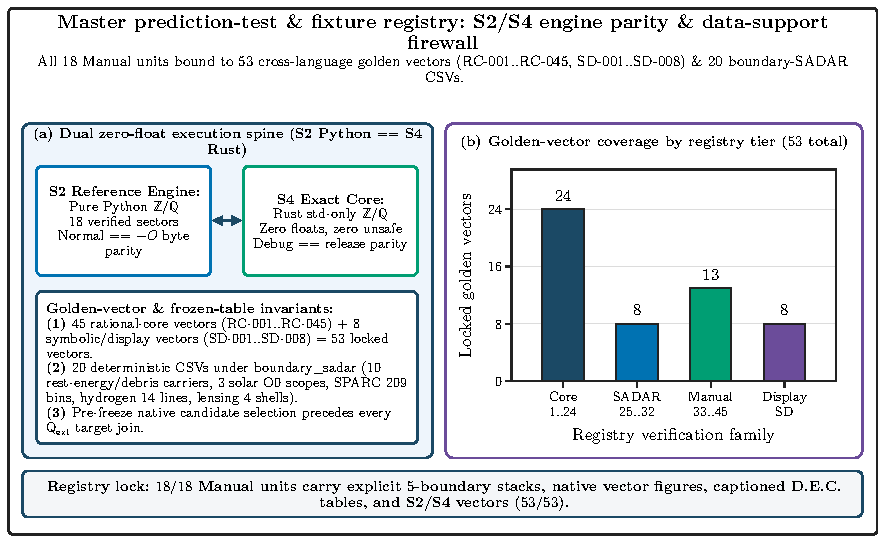
\includegraphics[width=0.92\linewidth,height=0.78\textheight,keepaspectratio]{figures/generated/registry-engine-coverage-atlas.pdf}
\caption{Dual S2 Python and S4 Rust zero-float reference-engine parity and fifty-three-vector registry coverage across all eighteen Manual units.}
\label{fig:manual-registry-engine-coverage}
\end{figure}

\begin{table}[H]
\centering
\caption{Master cross-language $53$-vector golden registry (\texttt{RC-001}--\texttt{RC-045}, \texttt{SD-001}--\texttt{SD-008}) and all $20$ frozen CSV artifacts under \texttt{manual/data/boundary\_sadar/}.}
\label{tab:manual-engine-dec-master-registry}
{\scriptsize
\begin{tabular}{>{\raggedright\arraybackslash}p{0.147\linewidth}>{\centering\arraybackslash}p{0.092\linewidth}>{\raggedright\arraybackslash}p{0.368\linewidth}>{\raggedright\arraybackslash}p{0.313\linewidth}}
\toprule
Vector IDs & Class & Ground-truth evaluator operation & Bound frozen CSV / source artifact \\
\midrule
\texttt{RC-001}--\texttt{RC-003} & $D0$ & One-node D.E.C. ($Z=8$), hinge-slide ($Z=7$), tunnelling clip ($6/7$) & \texttt{manual/\allowbreak{}data/\allowbreak{}dec/\allowbreak{}dec\_\allowbreak{}one\_\allowbreak{}node\_\allowbreak{}ledger\_\allowbreak{}example.csv}, \texttt{dec\_\allowbreak{}hinge\_\allowbreak{}slide\_\allowbreak{}example.csv}, \texttt{field\_\allowbreak{}tunnelling\_\allowbreak{}hinge\_\allowbreak{}slide\_\allowbreak{}window\_\allowbreak{}clip.csv} \\
\texttt{RC-004}--\texttt{RC-008} & $D0$ & AFC flux antisymmetry, $Q_4$ Hamming--1, $RD$/$\mathrm{RCD}$, relational cadence/lag, finite Stokes cut balance & Main \texttt{03\_\allowbreak{}afc\_\allowbreak{}basis}, \texttt{06\_\allowbreak{}field}, \texttt{06\_\allowbreak{}wave\_\allowbreak{}state\_\allowbreak{}relational\_\allowbreak{}time} exact algebraic oracles \\
\texttt{RC-033}, \texttt{SD-001}--\texttt{SD-002} & $D0$ & \S2 \texttt{dec\_\allowbreak{}native\_\allowbreak{}closure\_\allowbreak{}wave\_\allowbreak{}fold} \& \texttt{sympy\_\allowbreak{}z4\_\allowbreak{}dft} (even real \& odd $\mathbb{Q}(i)$ modes) & \texttt{native\_\allowbreak{}closure\_\allowbreak{}wave\_\allowbreak{}dec\_\allowbreak{}walk.csv}, \texttt{manual/\allowbreak{}data/\allowbreak{}native\_\allowbreak{}closure\_\allowbreak{}wave/\allowbreak{}harmonic\_\allowbreak{}reconstruction.csv} \\
\texttt{RC-009}--\texttt{RC-010}, \texttt{RC-034} & $D0$ & \S3 Awareness update, period-$6$ delay mindfulness, \texttt{dec\_\allowbreak{}awareness\_\allowbreak{}matched\_\allowbreak{}operativity} (cuts $23..34$) & \texttt{awareness\_\allowbreak{}operativity\_\allowbreak{}dec\_\allowbreak{}walk.csv}, \texttt{manual/\allowbreak{}scripts/\allowbreak{}aod\_\allowbreak{}awareness.py} \\
\texttt{RC-025}, \texttt{RC-026} & $D0$ & \S4 \texttt{dec\_\allowbreak{}chiral\_\allowbreak{}flip\_\allowbreak{}walk} ($Z=11\to7$, $T=6/7$) \& \texttt{dec\_\allowbreak{}two\_\allowbreak{}carrier\_\allowbreak{}chiral\_\allowbreak{}stokes} ($+4-4=0$) & \texttt{dec\_\allowbreak{}chiral\_\allowbreak{}flip\_\allowbreak{}continuous\_\allowbreak{}walk.csv} \\
\texttt{RC-045} & $D0$ & \S4/Core \texttt{ternary\_\allowbreak{}swar\_\allowbreak{}and\_\allowbreak{}trit\_\allowbreak{}ratio}: 2-bit/4-bit SWAR dwell burn, carry-barrier hinges, \texttt{TritWord}, \texttt{Trit2MicroRatio}, \texttt{TritRatio} & \texttt{manual/\allowbreak{}engine/\allowbreak{}ternary.py}, \texttt{crates/\allowbreak{}aod-core/\allowbreak{}src/\allowbreak{}ternary.rs} \\
\texttt{RC-035} & $D0$ & \S5 \texttt{dec\_\allowbreak{}cell\_\allowbreak{}measures\_\allowbreak{}staircase\_\allowbreak{}fold} ($Q_4$ 4-cell, 2D/4D staircase-to-$\pi$ \texttt{TritRatio}, fold chain-map) & \texttt{cell\_\allowbreak{}measures\_\allowbreak{}staircase\_\allowbreak{}fold\_\allowbreak{}dec.csv} \\
\texttt{RC-021}--\texttt{RC-024}, \texttt{SD-006}, \texttt{RC-036} & $D0$ & \S6 Typed float/bool/token rejection, MAP-21 \texttt{i128} variance, half-ULP enclosure, \texttt{dec\_\allowbreak{}typed\_\allowbreak{}maps\_\allowbreak{}exact\_\allowbreak{}laws} & \texttt{typed\_\allowbreak{}map\_\allowbreak{}joint\_\allowbreak{}law\_\allowbreak{}ledger.csv}, \texttt{manual/\allowbreak{}engine/\allowbreak{}numeric.py}, \texttt{manual/\allowbreak{}data/\allowbreak{}mapping\_\allowbreak{}error/\allowbreak{}mapping\_\allowbreak{}error.json} \\
\texttt{RC-017}--\texttt{RC-019}, \texttt{SD-003}, \texttt{RC-037} & $D0/O0$ & \S7 Cs-133 SI bridge, signed advance, H-maser mean, cyclotomic $\mathbb{Z}_{12}$, \texttt{dec\_\allowbreak{}temporal\_\allowbreak{}si\_\allowbreak{}bridge\_\allowbreak{}bounds} & \texttt{temporal\_\allowbreak{}si\_\allowbreak{}bridge\_\allowbreak{}dec\_\allowbreak{}ledger.csv}, \texttt{manual/\allowbreak{}data/\allowbreak{}temporal\_\allowbreak{}metrology/\allowbreak{}exact\_\allowbreak{}fixtures.json}, \texttt{report.json} \\
\texttt{RC-030} & $D0$ & \S8 \texttt{frg\_\allowbreak{}dimonhexon\_\allowbreak{}double\_\allowbreak{}slit\_\allowbreak{}ring} ($11$-bin $C_6$ path-pair generator, $410+38=448$, $\sum m=6$) & \texttt{dimonhexon\_\allowbreak{}double\_\allowbreak{}slit\_\allowbreak{}ring\_\allowbreak{}paths.csv} \\
\texttt{RC-038} & $D0$ & \S8 \texttt{dec\_\allowbreak{}short\_\allowbreak{}window\_\allowbreak{}rcd\_\allowbreak{}clipping} ($12$-pair $p^D+Q^D=3RD$ conservation, window-$9$ surplus $X=9$ vs $C_6=18$; $8$-row CSV $1:2:9$ $X=3$ vs $C_8=24$) & \texttt{short\_\allowbreak{}window\_\allowbreak{}rcd\_\allowbreak{}dec\_\allowbreak{}ledger.csv} \\
\texttt{RC-027} & $D0$ & \S9 \texttt{sadar\_\allowbreak{}pp\_\allowbreak{}tau\_\allowbreak{}five\_\allowbreak{}boundary} (sterile cut-$58$, raw $28=11+17$, unique $1:2:9_{\mathrm{yro}}$, $50$-microslot rotor $(650,703,1147)/2500\to(19/50,31/50)$) & \texttt{tau\_\allowbreak{}five\_\allowbreak{}boundary\_\allowbreak{}sadar\_\allowbreak{}trace.csv} \\
\texttt{RC-011}, \texttt{SD-004}--\texttt{SD-005} & $D0/O0$ & \S9 \texttt{higgs\_\allowbreak{}trace\_\allowbreak{}score\_\allowbreak{}and\_\allowbreak{}freeze} ($15616/125$ GeV) \& \texttt{higgs\_\allowbreak{}lhc\_\allowbreak{}rounded\_\allowbreak{}display} (CMS/ATLAS 6dp half-even) & \texttt{manual/\allowbreak{}data/\allowbreak{}higgs/\allowbreak{}higgs\_\allowbreak{}trace\_\allowbreak{}score\_\allowbreak{}formula.md}, \texttt{higgs\_\allowbreak{}external\_\allowbreak{}lhc\_\allowbreak{}mass\_\allowbreak{}comparison\_\allowbreak{}after\_\allowbreak{}freeze.csv} \\
\texttt{RC-028} & $D0$ & \S9 \texttt{sadar\_\allowbreak{}hadron\_\allowbreak{}debris\_\allowbreak{}and\_\allowbreak{}higgs\_\allowbreak{}saddle} ($3:2:6/8/10$ Ditrion debris \& $20$-candidate $3:3:7_{\mathrm{yro}}$ $\mathsf{C}_6/\mathsf{C}_8$ saddle) & \texttt{higgs\_\allowbreak{}baryon\_\allowbreak{}overlap\_\allowbreak{}saddle\_\allowbreak{}scan.csv} \\
\texttt{RC-029}, \texttt{SD-007} & $D0/\mathsf{Q}_{\mathrm{ext}}$ & \S9/App. B \texttt{sadar\_\allowbreak{}rest\_\allowbreak{}energy\_\allowbreak{}atlas} ($10$ carriers, $8160$ span, $9104$ closures) \& \texttt{sadar\_\allowbreak{}rest\_\allowbreak{}energy\_\allowbreak{}qext} (BIPM SI $K_{\mathrm{ext}}$) & \texttt{rest\_\allowbreak{}energy\_\allowbreak{}sadar\_\allowbreak{}debris\_\allowbreak{}atlas.csv} \\
\texttt{RC-031}, \texttt{RC-039} & $D0$ & \S10 \texttt{hydrogen\_\allowbreak{}shell\_\allowbreak{}series\_\allowbreak{}exact} \& \texttt{dec\_\allowbreak{}hydrogen\_\allowbreak{}shell\_\allowbreak{}wavelet\_\allowbreak{}step} (exact Balmer/Lyman/Paschen ratios) & \texttt{hydrogen\_\allowbreak{}shell\_\allowbreak{}exact\_\allowbreak{}series.csv}, \texttt{hydrogen\_\allowbreak{}shell\_\allowbreak{}dec\_\allowbreak{}transitions.csv} \\
\texttt{RC-032} & $D0$ & \S11 \texttt{scoped\_\allowbreak{}wire\_\allowbreak{}and\_\allowbreak{}moving\_\allowbreak{}boundary} ($8-3+2=7$ \& $4$-cut $1:2:6$ wire-electron walk $4\to4\to8\to13$) & \texttt{scoped\_\allowbreak{}wire\_\allowbreak{}and\_\allowbreak{}moving\_\allowbreak{}boundary\_\allowbreak{}walk.csv} \\
\texttt{RC-040} & $O0$ & \S12 \texttt{dec\_\allowbreak{}solar\_\allowbreak{}o0\_\allowbreak{}boundary\_\allowbreak{}audit} (exact Hg/bend/red residuals behind \texttt{HOLD\_\allowbreak{}MISSING\_\allowbreak{}NATIVE\_\allowbreak{}SOLAR\_\allowbreak{}PRODUCER}) & \texttt{solar\_\allowbreak{}o0\_\allowbreak{}boundary\_\allowbreak{}dec\_\allowbreak{}audit.csv} \\
\texttt{RC-012}--\texttt{RC-013}, \texttt{RC-041} & $G3/D0$ & \S13 Brownian MSB-$x$, run-tumble LSB-$x$, \texttt{dec\_\allowbreak{}run\_\allowbreak{}tumble\_\allowbreak{}q4\_\allowbreak{}stepper} ($21$-tick $Q_4\to\mathbb{Z}^3$ walk, tick-$16$ closure) & \texttt{run\_\allowbreak{}tumble\_\allowbreak{}q4\_\allowbreak{}dec\_\allowbreak{}walk.csv}, \texttt{manual/\allowbreak{}data/\allowbreak{}brownian/\allowbreak{}octant\_\allowbreak{}delta3.csv}, \texttt{run\_\allowbreak{}tumble\_\allowbreak{}octant\_\allowbreak{}delta3.csv} \\
\texttt{RC-015}--\texttt{RC-016}, \texttt{SD-008} & $G0$ & \S13 \texttt{sparc\_\allowbreak{}exact\_\allowbreak{}bin\_\allowbreak{}eval} (per-bin) \& \texttt{sparc\_\allowbreak{}pooled\_\allowbreak{}primary\_\allowbreak{}exact} ($209$ bins, exact $MAPE_U=26.57055342\%$ from $230/228$ digits) & \texttt{sparc\_\allowbreak{}pooled\_\allowbreak{}primary\_\allowbreak{}exact.csv}, \texttt{manual/\allowbreak{}data/\allowbreak{}derived/\allowbreak{}sparc\_\allowbreak{}five\_\allowbreak{}galaxy\_\allowbreak{}per\_\allowbreak{}bin.csv} \\
\texttt{RC-020}, \texttt{RC-042} & $L0/L1/L2$ & \S14 SWELLS K1 $\sum m=8$ \& Tau $1/100$ non-conflation, \texttt{dec\_\allowbreak{}lensing\_\allowbreak{}ray\_\allowbreak{}chiral\_\allowbreak{}delta3} ($4$-shell FRG walk, $3$ flips) & \texttt{lensing\_\allowbreak{}ray\_\allowbreak{}chiral\_\allowbreak{}dec\_\allowbreak{}walk.csv}, \texttt{manual/\allowbreak{}data/\allowbreak{}lensing/\allowbreak{}swells\_\allowbreak{}k1\_\allowbreak{}thetaE\_\allowbreak{}delta3\_\allowbreak{}scores.csv} \\
\texttt{RC-014}, \texttt{RC-043}, \texttt{RC-044} & $D0/G3$ & App. A exact rational cycle shedding (\texttt{cycle\_\allowbreak{}shedding\_\allowbreak{}step}, \texttt{dec\_\allowbreak{}cycle\_\allowbreak{}shedding\_\allowbreak{}exact\_\allowbreak{}summary}) \& App. C \texttt{dec\_\allowbreak{}coordinate\_\allowbreak{}phase\_\allowbreak{}3d\_\allowbreak{}walk} & \texttt{cycle\_\allowbreak{}shedding\_\allowbreak{}exact\_\allowbreak{}rational\_\allowbreak{}summary.csv}, \texttt{coordinate\_\allowbreak{}phase\_\allowbreak{}3d\_\allowbreak{}dec\_\allowbreak{}walk.csv} \\
\bottomrule
\end{tabular}
}
\end{table}
